% Contribution fragment only. Merge into the team ACM report.
% Requires graphicx and the supplied BibTeX entries.
\subsection{Draft Entity Relationship Model}
Our draft ER diagram starts with a customer and their investment portfolio, which is the collection of investments they own. A Holding connects a Portfolio to an ETF, a fund traded on a stock exchange, and records its portfolio weight and observation date. This separates the customer's investment mix from the allocation reported for each fund. ETFIdentifier also stores the identifier scheme and, where needed, exchange context, so we do not rely on a ticker alone to identify an ETF.

The main refinement is AllocationSnapshot. Each snapshot describes one ETF, one date and one allocation dimension, either sector or geography. It contains AllocationEntry records, each connecting a category to its disclosed percentage. A new observation creates a new snapshot rather than replacing the previous percentages. SourceDocument records the captured provider document or webpage, its URL and retrieval time. ClassificationScheme gives categories their stated classification context, when the source provides it. Keeping the allocation basis and coverage notes also helps us interpret disclosures that exclude cash or show only part of a fund \cite{vfv_disclosure,xic_disclosure}.

FIBO provides relevant building blocks, but their meaning needs care. Its fund-classification concepts describe the type of fund, and definesAllocations links investment policy to allocation limitations \cite{fibo_funds}. We therefore represent a published allocation as an observation, rather than as a policy. FIBO's weighted-basket and date concepts are also candidates for reuse, subject to their ontology restrictions \cite{fibo_baskets,fibo_dates}. Browne et al. already demonstrate FIBO-based reporting of dated fund information and allocation summaries \cite{browne2017}. Our proposed contribution is narrower: an explicit pattern connecting a provider-published ETF allocation to its date, entries, categories, classification context and source. This is a proposed integration gap, not a claim that FIBO lacks weights or dates.

The model supports portfolio exposure estimates by combining holding weights with compatible disclosed category weights. The result should retain the selected snapshot dates and sources. We will evaluate the later relational and semantic versions with the same competency questions, using one or two fictional portfolios and two or three ETFs. Full holdings reconstruction, return prediction and portfolio optimisation remain outside this project.

% Place this figure on the diagram page of the final report.
\begin{figure*}[p]
\centering
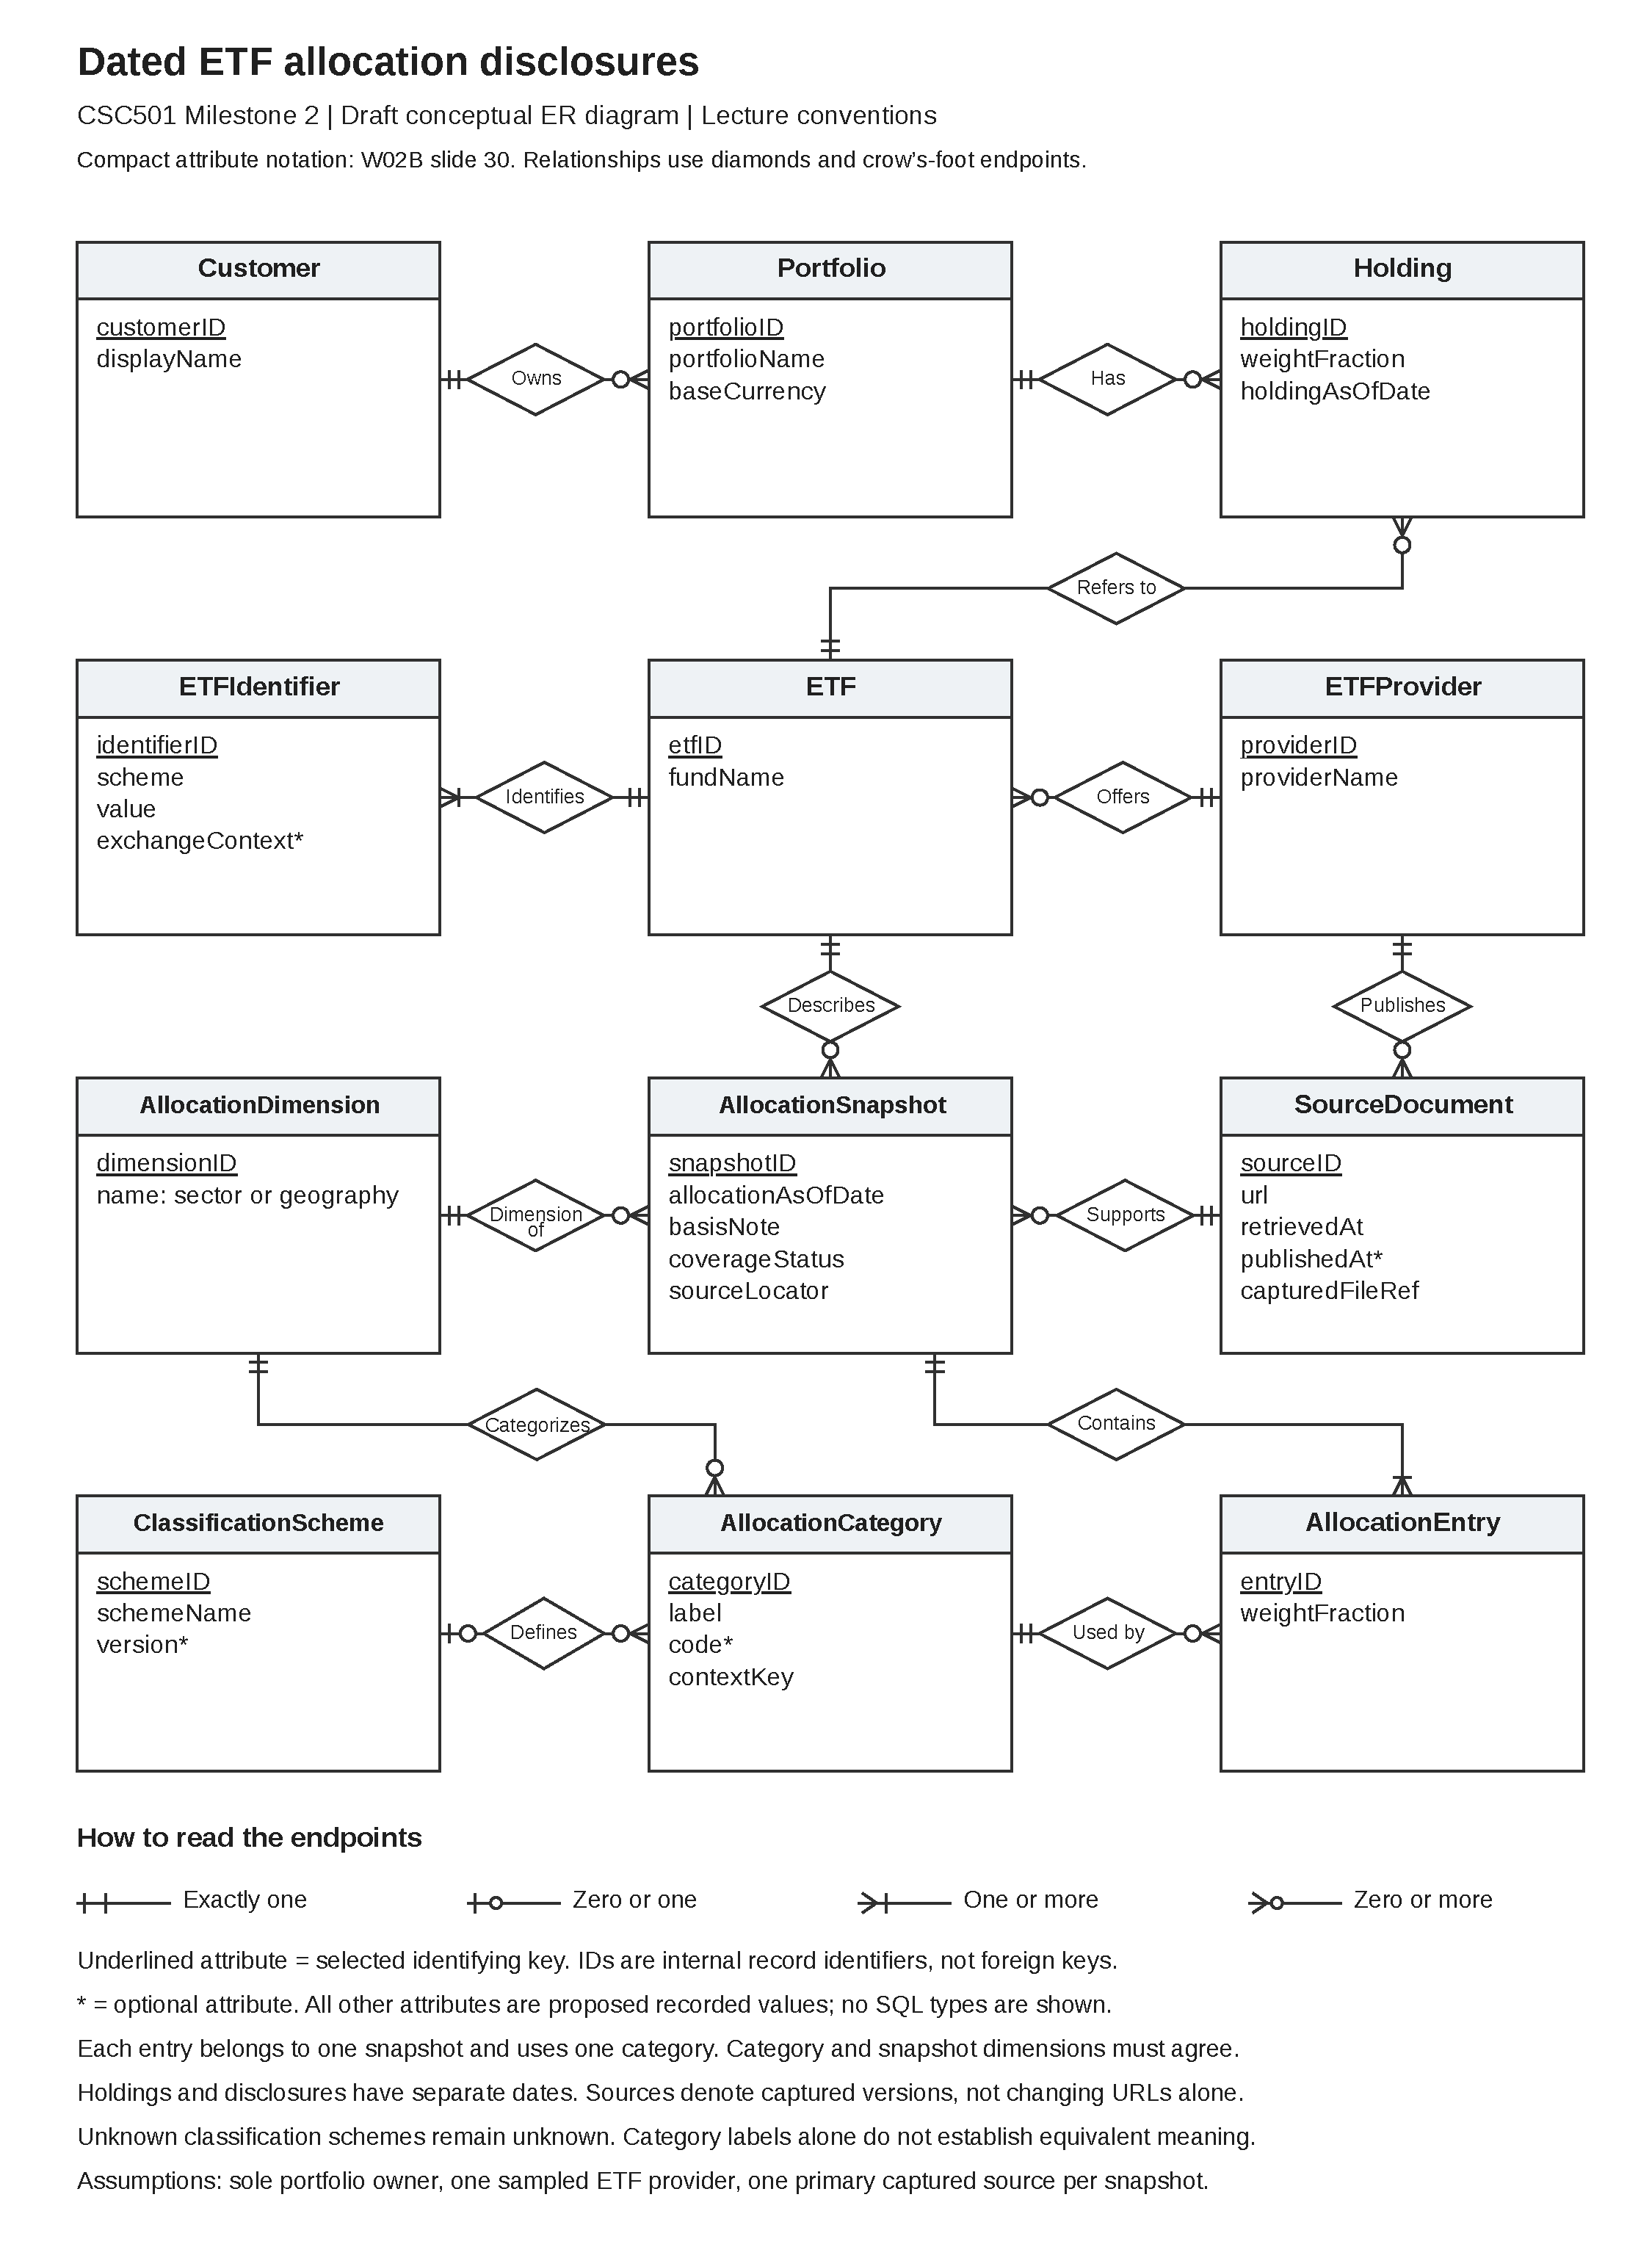
\includegraphics[width=0.96\textwidth,height=0.85\textheight,keepaspectratio]{CSC501_M2_Taimoor_ERD_Connectors.pdf}
\caption{Draft conceptual ER diagram for dated ETF allocation disclosures. Holding records the customer's ETF weight at a portfolio observation date; AllocationSnapshot records a provider's disclosure date. The disclosure pattern connects an ETF, source, dimension, entries and category context. Cardinalities describe the small course dataset and are not final OWL restrictions.}
\label{fig:etf-allocation-erd}
\end{figure*}